\documentclass{standalone}

\usepackage{pgfplots}

\pgfplotsset{compat=newest}

\begin{document}
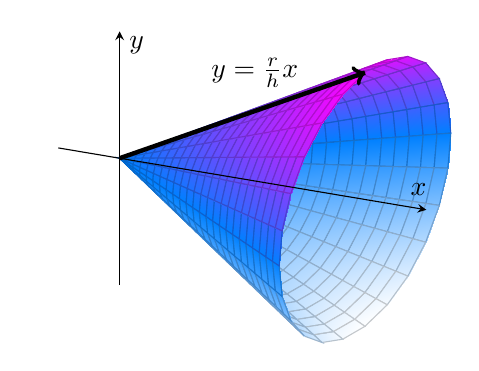
\begin{tikzpicture}
    \begin{axis}[axis lines=center, axis on top, xlabel=$x$, zlabel=$y$, y axis line style={draw=none}, tick style={draw=none}, xticklabel=\empty, yticklabel=\empty, zticklabel=\empty, xmin=-1, xmax=5]
        % cone
        \addplot3[domain=0:4, y domain=0:2*pi, surf, shader=faceted interp, colormap/cool]({x}, {x*sin(deg(y))},{x*cos(deg(y))});
        % line
        \addplot3[domain=0:4, ultra thick, ->]({x}, 0, {x}) node[left, xshift=-2em] {$y=\frac{r}{h}x$};
    \end{axis}
\end{tikzpicture}
\end{document}
